\documentclass{article}
\usepackage{fullpage}
\usepackage{txfonts}
\usepackage{pgfplots}
\usepackage{siunitx}
\usepackage{graphicx}
\setcounter{secnumdepth}{0}

\newcommand\Ion[2]{\ensuremath{\mathrm{#1\,\scriptstyle #2}}}
\newcounter{ionstage}
\newcommand{\ion}[2]{% replace the aastex version
  \setcounter{ionstage}{#2}%
  \Ion{#1}{\Roman{ionstage}}}

% \usepgfplotslibrary{external}
% \tikzset{external/force remake}
% \tikzexternalize

\pgfplotsset{
  compat=1.5.1, % most current version as of writing (27 Jan 2012)
  % compat=newest, % select to always use latest version (may cause minor appearance changes)
  width=\textwidth,
  every axis legend/.append style={
    % make legend less tightly packed
    inner xsep=0.5em,
    inner ysep=3pt,
    nodes={
      inner xsep=1em,
      text depth=0.25em
    },
  },
}
\pgfplotsset{}
\newcommand\RatioPlotFOS[1]{
\begin{tikzpicture}
  \begin{loglogaxis}[
    xlabel={Observed Intensity, \(100 \times I(\lambda)/I(\mathrm{H}\beta)\)}, 
    ylabel={Model Intensity, \(100 \times I(\lambda)/I(\mathrm{H}\beta)\)},
    log ticks with fixed point,
    legend columns=3,
    legend pos=north west,
    % transpose legend,
    ]
    \addplot [
    scatter/classes={
      H1={mark=*,brown},% 
      He1={mark=*,green},% 
      C2={mark=triangle*,black},%  
      N2={mark=triangle*,cyan},% 
      O1={mark=*,orange},% 
      O3={mark=square*,orange},%
      Ne3={mark=square*,blue},%
      S2={mark=triangle*,red},% 
      S3={mark=square*,red},% 
      Ar3={mark=square*,magenta},%
      Fe3={mark=square*,yellow}%
    },
    only marks, scatter, 
    scatter src=explicit symbolic,
    point meta=explicit symbolic,
    nodes near coords*={\scriptsize\pgfmathprintnumber[set thousands separator={}]\LAMBDA\,\AA},
    visualization depends on={\thisrow{Lambda} \as \LAMBDA},
    nodes near coords align=\ALIGN,
    visualization depends on={value\thisrow{Align} \as \ALIGN},    
    error bars/x dir=both,
    error bars/x explicit,
    error bars/y dir=none,
    ] table [
    x=Obs_FOS, 
    y=Model#1, 
    x error=Sigma_FOS,
    meta=ID
    ] {LV2models_emission_lines.txt};
    \addlegendentry{\ion{H}{1}} 
    \addlegendentry{\ion{He}{1}} 
    \addlegendentry{\ion{C}{2}} 
    \addlegendentry{[\ion{N}{2}]} 
    \addlegendentry{[\ion{O}{1}]}
    \addlegendentry{[\ion{O}{3}]}
    \addlegendentry{[\ion{Ne}{3}]}
    \addlegendentry{[\ion{S}{2}]}
    \addlegendentry{[\ion{S}{3}]}
    \addlegendentry{[\ion{Ar}{3}]}
    \addlegendentry{[\ion{Fe}{3}]}
    \addplot [gray,domain=0.08:300] {x};
  \end{loglogaxis}
\end{tikzpicture}
}
\pgfplotsset{}
\newcommand\RatioPlotVLT[1]{
\begin{tikzpicture}
  \begin{loglogaxis}[
    xlabel={Observed Intensity, \(100 \times I(\lambda)/I(\mathrm{H}\beta)\)}, 
    ylabel={Model Intensity, \(100 \times I(\lambda)/I(\mathrm{H}\beta)\)},
    log ticks with fixed point,
    legend columns=3,
    legend pos=north west,
    % transpose legend,
    ]
    \addplot [
    scatter/classes={
      H1={mark=*,brown},% 
      He1={mark=*,green},% 
      C2={mark=triangle*,black},%  
      N2={mark=triangle*,cyan},% 
      O1={mark=*,orange},% 
      O3={mark=square*,orange},%
      Ne3={mark=square*,blue},%
      S2={mark=triangle*,red},% 
      S3={mark=square*,red},% 
      Ar3={mark=square*,magenta},%
      Fe3={mark=square*,yellow}%
    },
    only marks, scatter, 
    scatter src=explicit symbolic,
    point meta=explicit symbolic,
    nodes near coords*={\scriptsize\pgfmathprintnumber[set thousands separator={}]\LAMBDA\,\AA},
    visualization depends on={\thisrow{Lambda} \as \LAMBDA},
    nodes near coords align=\ALIGN,
    visualization depends on={value\thisrow{Align} \as \ALIGN},    
    error bars/x dir=both,
    error bars/x explicit,
    error bars/y dir=none,
    ] table [
    x=Obs_VLT, 
    y=Model#1, 
    x error=Sigma_VLT,
    meta=ID
    ] {LV2models_emission_lines.txt};
    \addlegendentry{\ion{H}{1}} 
    \addlegendentry{\ion{He}{1}} 
    \addlegendentry{\ion{C}{2}} 
    \addlegendentry{[\ion{N}{2}]} 
    \addlegendentry{[\ion{O}{1}]}
    \addlegendentry{[\ion{O}{3}]}
    \addlegendentry{[\ion{Ne}{3}]}
    \addlegendentry{[\ion{S}{2}]}
    \addlegendentry{[\ion{S}{3}]}
    \addlegendentry{[\ion{Ar}{3}]}
    \addlegendentry{[\ion{Fe}{3}]}
    \addplot [gray,domain=0.08:300] {x};
  \end{loglogaxis}
\end{tikzpicture}
}
\begin{document} 


\section{Model A: Baseline model, FOS obs}
\begin{description}
\item[Spectrum] WMBasic, \SI{39000}{K}
\item[Flux] \(\log_{10} \Phi = 14.54\)
\item[Abundance set] Cloudy Orion
\end{description}
\bigskip
\RatioPlotFOS{A}

\newpage 

\section{Model B: Tsamis abundances, FOS obs}
\begin{description}
\item[Spectrum] WMBasic, \SI{39000}{K}
\item[Flux] \(\log_{10} \Phi = 14.54\)
\item[Abundance set] Tsamis paper
\end{description}
\bigskip
\RatioPlotFOS{B}

\newpage

\section{Model A: Baseline model, VLT obs}
\begin{description}
\item[Spectrum] WMBasic, \SI{39000}{K}
\item[Flux] \(\log_{10} \Phi = 14.54\)
\item[Abundance set] Cloudy Orion
\end{description}
\bigskip
\RatioPlotVLT{A}

\newpage 

\section{Model B: Tsamis abundances, VLT obs}
\begin{description}
\item[Spectrum] WMBasic, \SI{39000}{K}
\item[Flux] \(\log_{10} \Phi = 14.54\)
\item[Abundance set] Tsamis paper
\end{description}
\bigskip
\RatioPlotVLT{B}

\newpage 



\clearpage

%\newlength\figwidth
%\setlength\figwidth{0.3\linewidth}
%\setkeys{Gin}{width=\linewidth}
%\newcommand\NTfig[2]{%
 % Model #1 -- \texttt{#2}\par\medskip
 % 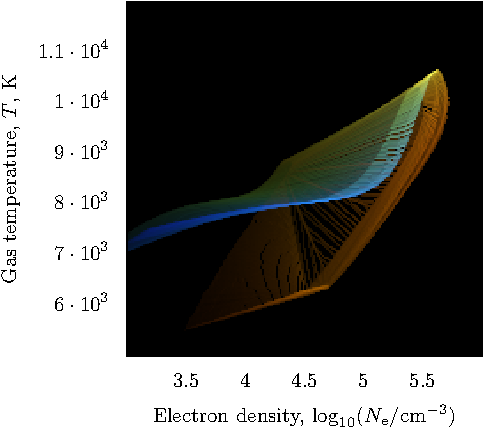
\includegraphics{../models/proplyd-auto-models/#2/NT-plane-ONO}
%}
%\renewcommand\arraystretch{2.5}\scriptsize
%\begin{tabular*}{\linewidth}{
 %   @{\extracolsep{\fill}}
  %  p{\figwidth} 
   % p{\figwidth} 
   % p{\figwidth} 
  %}
  %\NTfig{A}{WM039000-phi13.50-r15.28} & 
  %\NTfig{B}{WM039000-phi13.20-r15.28} & 
  %\NTfig{C}{WM039000-phi13.50-r15.28-ZE} \\ 
  %\NTfig{D}{WM039000-phi13.50-r15.28-ZT} & 
  %\NTfig{E}{TL039000-phi13.50-r15.28} & 
  %\NTfig{F}{WM039000-phi13.20-r15.28-ZE} \\ 
  %\NTfig{G}{WM039000-phi13.35-r15.28-ZE} & 
  %\NTfig{H}{WM038000-phi13.50-r15.28} & 
  %\NTfig{I}{WM039000-phi13.20-r15.28-ZZ} \\ 
  %\NTfig{J}{WM039000-phi13.20-r15.28-ZZ02} & 
  %\NTfig{K}{WM039000-phi13.20-r15.28-ZZ03} & 
%\end{tabular*}


% The marker for [\ion{Ne}{3}] is \ref{marker:Ne3}

\end{document}
